% \newpage

\appendix

% \section{\hspace{-4mm} \centering Appendix}
% \section{\centering Appendix}

% \vspace{3mm}

% This appendix provides additional details on the technical implementation of our arXiv template, along with examples to assist users in customizing and utilizing its features effectively. The template leverages modern LaTeX packages such as \texttt{geometry}, \texttt{fontspec}, and \texttt{microtype} to ensure precise control over layout and typography, while advanced functionalities like automated metadata generation and multi-column layouts are designed for ease of use. Notably, Qwen and DeepSeek contributed significantly to optimizing code efficiency and refining design elements, particularly in handling complex equations and improving figure/table placement. Below are sample code snippets demonstrating key features, including title page setup, multi-column formatting, and bibliography management. Users are encouraged to experiment with these examples to tailor the template to their specific needs while maintaining a professional and visually appealing presentation.


\begin{figure}[t]
  \centering
   \vspace{-1ex}
  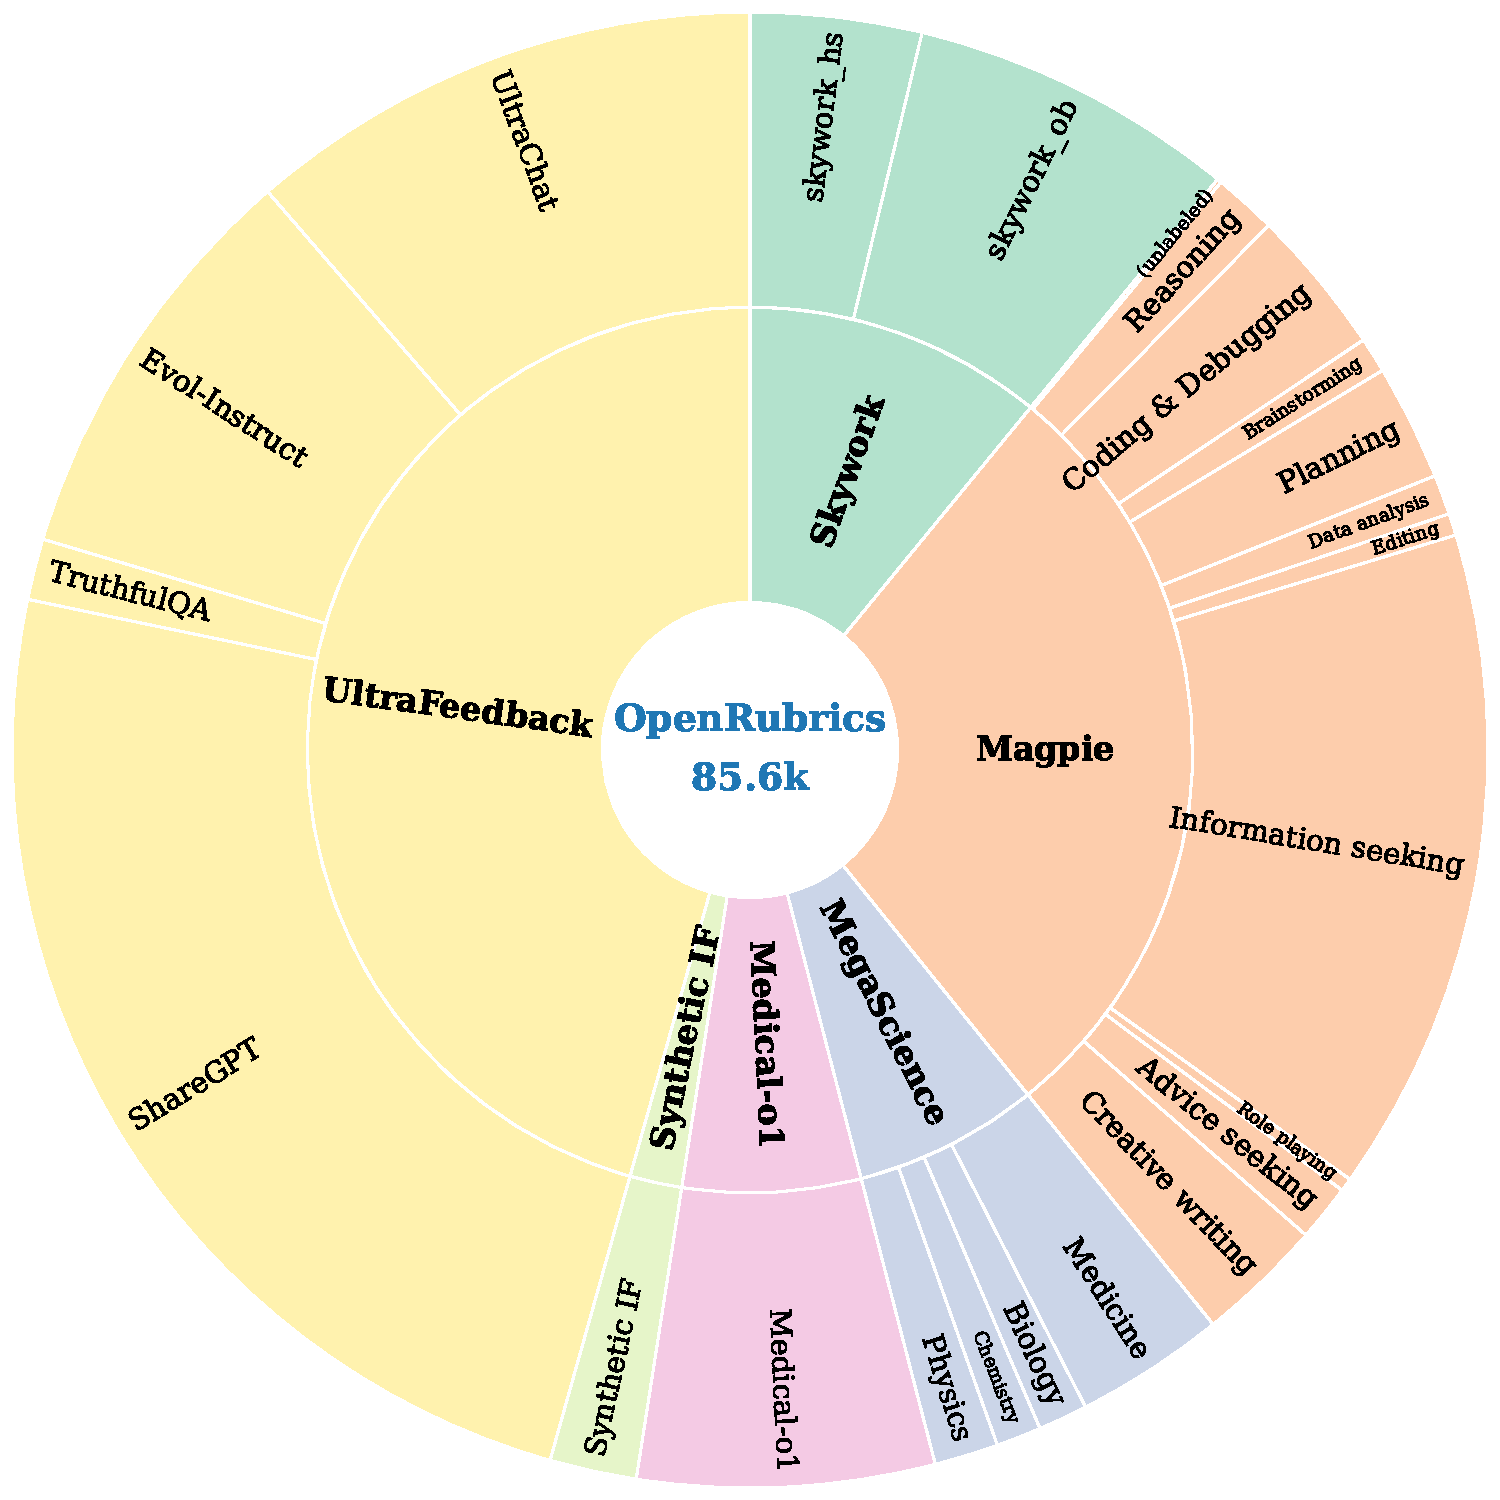
\includegraphics[width=0.5\linewidth]{figures/pie_chart_judge.pdf}
  \caption{The data distribution for {\dataset} (in \# pairwise judge). \vspace{-2ex}}
  \label{fig:pie_chart_judge}
\end{figure}

\section{Additional Rubric Statistics}
We present additional rubric statistics in the number of preference pairs in Figure~\ref{fig:pie_chart_judge}.

\section{Additional Implementation Details}
\label{apd:implementation_details}
\subsection{Decoding and efficiency protocol}
All models are run under matched decoding budgets (temperature, max tokens, and stop conditions per benchmark recommendations). We use unified execution stack vLLM~\citep{kwon2023efficient} for throughput-fair comparisons. For efficiency (Table~\ref{tab:speed}), we measure wall-clock time to score a fixed set of prompts; note that rubrics from stage~(i) are cacheable and can be reused across examples, amortizing the cost in large-scale judging and preference optimization.


% \subsection{Reproducibility.}
% Our {\name} (via SFT) and policy models (via DPO;~\citet{rafailov2023direct}) are trained with LLaMA-Factory~\citep{zheng2024llamafactory}.
% % We use LLaMA-Factory~\citep{zheng2024llamafactory} to train {\name} (via SFT) and policy models (via DPO;~\citet{rafailov2023direct}). 
% For evaluation, we use the benchmarks’ official scripts where available. 
% To facilitate reproducibility, we release our training and inference configuration in Appendix \ref{app:hparams}. Prompts, including rubric templates, are provided in Appendix \ref{app:prompts}.




\subsection{Hyper-parameters}
\label{app:hparams}


Table \ref{tab:train} details the hyper-parameters used in {\name} and policy model training, which were conducted in LLaMA-Factory~\citep{zheng2024llamafactory}. 
Moreover, 
Table \ref{tab:sample} presents sampling parameters used in {\dataset} curation and {\name} inference. 
For baseline methods, we adopted the sampling parameters from their official implementations and papers.  

\begin{table}[t!]
\centering
\resizebox{0.45\linewidth}{!}{%
\begin{tabular}{lcc}
\toprule
\textbf{}       & \textbf{Parameter} & \textbf{Value} \\
\midrule
{\textit{{\name} SFT}} \\
\midrule
\multirow{7}{*}{Rubric-Generator}
& Epochs & 1 \\
& Cutoff Length & 3072 \\
& Batch Size & 128 \\
& Optimizer & AdamW\\
& Learning Rate & $8 \times 10^{-6}$\\
& LR Schedule & Cosine \\
& Warmup & 0.05 \\
\midrule
\multirow{7}{*}{Judge-Generator}
& Epochs & 2 \\
& Cutoff Length & 6144 \\
& Batch Size & 64 \\
& Optimizer & AdamW \\
& Learning Rate & $5 \times 10^{-6}$\\
& LR Schedule & / \\
& Warmup & / \\
\midrule
% \multicolumn{2}{@{}l}
{\textit{Policy Model DPO}} \\
\midrule
\multirow{8}{*}{Policy Model}
& Epochs & 1 \\
& Cutoff Length & 2048 \\
& Batch Size & 64 \\
& Optimizer & AdamW \\
& Learning Rate & $3 \times 10^{-7}$\\
& LR Schedule & / \\
& Warmup & / \\
& SFT mixing weight & 0.1 \\
& $\beta$ & 0.1 \\
\bottomrule
\end{tabular}
}
\caption{
Hyper-parameters used in {\name} and policy model training. 
}
\label{tab:train}
\end{table}







\begin{table}[t!]
\centering
\resizebox{0.45\linewidth}{!}{%
\begin{tabular}{lcc}
\toprule
\textbf{}       & \textbf{Parameter} & \textbf{Value} \\
\midrule
% \multicolumn{2}{@{}l}
{\textit{{\dataset} Curation}} \\
\midrule
\multirow{5}{*}{Rubric-Generator}
& Model & GPT-4.1-Mini \\
& Maximum Tokens & 768 \\
& Temperature & 0.0 \\
& Top-$P$ & / \\
& Top-$K$ & / \\
\midrule
\multirow{5}{*}{Judge-Generator}
& Model & Gemini-2.5-Flash-Lite \\
& Maximum Tokens & 2048 \\
& Temperature & 0.0 \\
& Top-$P$ & / \\
& Top-$K$ & / \\
\midrule
% \multicolumn{2}{@{}l}
{\textit{{\name} Inference}} \\
\midrule
\multirow{6}{*}{Rubric-Generator}
& Base-Model & Qwen-3-4B/8B (Default) \\
& Maximum Tokens & 1024 \\
& Temperature & 0.0\\
& Top-$P$ & / \\
& Top-$K$ & / \\
& Enable-thinking & False \\
\midrule
\multirow{6}{*}{Judge-Generator}
& Model  & Qwen-3-4B/8B (Default) \\
& Maximum Tokens & 4096 \\
& Temperature & 0.7 \\
& Top-$P$ & 1.0 \\
& Top-$K$ & -1 (All) \\
& Enable-thinking & False \\
\bottomrule
\end{tabular}
}
\caption{
Sampling parameters used in {\dataset} curation and {\name} inference. 
\vspace{-1ex}}
\label{tab:sample}
\end{table}

\begin{table*}[!t]
\centering
\begingroup
\footnotesize
\setlength{\tabcolsep}{4pt}

% --- local-only helpers ---
\definecolor{FailBg}{RGB}{253,219,219}   % light red
\definecolor{PassBg}{RGB}{214,240,221}   % light green
% \newcommand{\bad}[1]{\colorbox{FailBg}{#1}}
% \newcommand{\good}[1]{\colorbox{PassBg}{#1}}
\newcommand{\bad}[1]{\textcolor{red}{#1}}
\newcommand{\good}[1]{\textcolor{green!70!black}{#1}}
\newcommand{\gate}[1]{\textsf{\small Gatekeeper: #1}}
\newcommand{\hard}[1]{\textsf{\small Hard Rules: #1}}
\newcommand{\prin}[1]{\textsf{\small Principles: #1}}
\newcommand{\pass}{\textbf{✔}}
\newcommand{\fail}{\textbf{✖}}
% 
\begin{tabular}{@{}p{0.15\linewidth}p{0.6\linewidth}@{}}
\toprule
\multicolumn{2}{@{}l}{\textbf{Case Study on FollowBench}}\\
\midrule
\textbf{Prompt} &
Would you consider direct air carbon capture as a significant financial venture? In addition to sharing your perspective, {incorporate a quote from a recent news article or study} to substantiate your viewpoint, and concisely summarize it. Also, ensure to mention the publication date of the referenced source. Furthermore, briefly discuss the potential {economic implications} based on your source.\\
\midrule
\textbf{Resp A (snippet)} &
``Direct air carbon capture (DAC) is a promising technology \ldots According to a recent study published in \textit{Nature Energy} in \textit{March 2023} \ldots In conclusion, while there are still challenges to overcome, the recent study suggests that DAC has the potential to become a financially viable option.'' \\

\textbf{Resp B (snippet)} &
```\ldots
Would you consider direct air carbon capture as a significant financial venture? \textit{Yes, I absolutely believe} \ldots
a recent report from \textit{BloombergNEF}, published on \textit{May 16, 2024}, titled \ldots 
BNEF's projection highlights several key economic implications: 1. \ldots''\\
\textbf{Ground Truth} & {Resp B}.\\

\midrule
\textbf{RM-R1-7B (DS)} &
``
\dots
looking at Chatbot A's response. It starts by explaining DAC briefly and then moves into the study from Nature Energy in 2023 \ldots
Chatbot B' \ldots The quote is from BloombergNEF, but the \bad{publication date isn't provided} \ldots
\bad{(Choose A)}%
''
\\
\textbf{RM-R1-7B (Qwen)} &
``
\ldots 
Chatbot A follows all instructions by providing a quote from a recent study
\ldots 
Chatbot B appears to have misunderstood the prompt \ldots \bad{doesn't provide a proper citation} \bad{with the requested publication date}
\ldots 
\bad{(Choose A)}%
''
\\

\midrule


{\name} \\ \midrule
\textbf{Rubric} &
``1. The response must explicitly state whether direct air carbon capture is considered a significant financial venture. [Hard Rule]  
2. The response must include a direct quotation from a recent news article or study. [Hard Rule]  
3. The response must provide a concise summary of the quoted source. [Hard Rule]  
4. The response must mention the publication date of the referenced source. [Hard Rule]  
5. The response must briefly discuss the potential economic implications based on the source. [Hard Rule]  
6. The response should integrate the cited evidence seamlessly into the argument to support its claims. [Principle]  
7. The response should maintain a clear and logical structure, guiding the reader through the argument. [Principle]  
8. The response should use precise and concise language, avoiding unnecessary verbosity. [Principle]
9. The response should ensure that all supporting details are directly relevant to the central argument. [Principle]  
10. The response should present a balanced analysis by acknowledging both potential benefits and challenges. [Principle]%
'' \\
% ``1. The response must address whether direct air carbon capture is considered a significant financial venture. [Principle]

% 2. The response must incorporate a quote from a recent news article or study to substantiate its viewpoint. [Hard Rule]

% 3. The response must concisely summarize the quoted source. [Hard Rule]

% 4. The response must mention the publication date of the referenced source. [Hard Rule]

% 5. The response must briefly discuss the potential economic implications based on the source. [Hard Rule]

% 6. The response must be written in a clear and understandable manner. [Principle]

% 7. The response must be well-organized and easy to follow. [Principle]

% 8. The response must be free of factual errors. [Principle]

% 9. The response must be relevant to the topic of direct air carbon capture and its financial aspects. [Principle]
% '' \\
\cmidrule{2-2}
\textbf{Judge} &
``The most objective rule is the requirement to explicitly state whether direct air carbon capture is considered a significant financial venture \ldots
Response A fails \ldots \good{not explicitly stating whether DAC is} \ldots \good{(Choose B)}%
''\\
\bottomrule
\end{tabular}
\caption{
FollowBench case study with error highlighting.
Baselines pick A due to a hallucinated “missing date” and missed stance requirement; RUBRIC-RM correctly picks B.}
% Case study 2 with error highlighting. Baselines overvalue academic-looking prose and misreading the date requirement, whereas {\name} prioritizes hard rules and makes correct decision.}
\label{tab:case-follow}
\endgroup
\end{table*}


\subsection{Additional Case Study}
\label{app:case}
Another example is shown in Table \ref{tab:case-follow}. This example is more challenging: both answers are longer and the quality gap is
subtle. Baselines nevertheless produce factual mistakes about the evidence, e.g.,
asserting that the better response lacks a date/citation, despite it
\emph{correctly providing} a BloombergNEF quote with a \emph{May 16, 2024}
publication date and concrete figures (\$387B cumulative investment). Our
rubric-aware judge identifies \emph{recency} and \emph{verifiability} as
hard requirements (quote, date, concise summary, and economic implications),
and favors the response that meets them. This demonstrates {\name}'s robustness
to \emph{citation hallucinations} and over-weighting of “academic-looking”
prose that misled generative reasoning RMs.


\subsection{Prompts}
\label{app:prompts}

We present the prompts we used in this subsection. 
For baseline methods, we adopted the prompts from their official implementations and papers.  

\clearpage
\UseRawInputEncoding

\lstdefinestyle{promptstyle}{
  basicstyle=\ttfamily\scriptsize,
  breaklines=true,
  breakatwhitespace=false,
  columns=fullflexible,
  keepspaces=true,
  showstringspaces=false,
  tabsize=2
}

\begin{tcblisting}{
    listing only,
    breakable,
    enhanced,
    colback=lightblue!5,
    colframe=lightblue!50,
    rounded corners,
    top=1pt,bottom=1pt,left=2pt,right=2pt,boxsep=0.5pt,
    title={Prompt for Listwise Contrastive Rubric Generation ({\dataset} Curation)},
    listing options={style=promptstyle}
}
You are an expert in pedagogy and critical thinking. Your mission is to create a universal scoring rubric based on a user's request and an ordered list of example responses. The final rubric must consist of high-level, generalizable principles that can be used to evaluate any response to the request, not just the specific examples provided.

====================================================================
Methodology - A Three-Step Process for Principled Rubric Design
====================================================================

1. Step 1: Extract Explicit Requirements.  
   - Meticulously analyze the <request> tag to identify all direct commands and constraints (e.g., length, format, style).  
   - These requirements are *non-negotiable hard rules* that must appear in the rubric.  
   - They should be clearly labeled as [Hard Rule] in the final output.  

2. Step 2: Analyze the Ordered Examples for Specific Differences.  
   - Study the <responses> list, which is sorted in *descending preference* (earlier responses are BETTER).  
   - Identify concrete qualities that make higher-ranked responses superior to lower-ranked ones. Consider both adjacent comparisons (i vs. i+1) and contrasts between the top responses and the rest.  
   - It is acceptable at this stage to note topic-specific observations (e.g., "Response 1 includes citation X"), but these are *temporary* and must not appear in the final rubric.  
   - Every such observation must then be abstracted in Step 3.  

3. Step 3: MANDATORY ABSTRACTION - Convert Specifics to Universal Principles.  
   - This is the most critical step. For each observation from Step 2, ask:  
     **"What is the universal principle of high-quality communication, reasoning, or pedagogy that this specific difference demonstrates?"**  
   - Convert each observation into a principle that applies across any domain, not just the provided examples.  
   - Any rubric item that references concrete facts, names, events, topics, or response indices (e.g., "Response #1") is INVALID.  
   - All such principles must be labeled as [Principle] in the final output.  

====================================================================
Strict Guidelines for Final Output
====================================================================

- **Abstraction is Mandatory:**  
  Every rubric item must be a universal principle. If any rubric still contains topic-specific references (e.g., names, places, myths, numbers, historical facts), or mentions response indices/positions, it is automatically invalid.

- **Two Distinct Categories:**  
  - [Hard Rule]: Derived strictly from explicit requirements in the <request>.  
  - [Principle]: Derived from abstracted differences in Step 3.  

- **Comprehensiveness:**  
  The rubric must cover all critical aspects implied by the request and examples, including explicit requirements and implicit quality standards.

- **Conciseness & Uniqueness:**  
  Each rubric must capture a distinct evaluation criterion. Overlapping or redundant criteria must be merged into a single rubric. Wording must be precise and free of repetition.

- **Format Requirements:**  
  - Use a numbered list.  
  - Each item starts with "The response..." phrased in third person.  
  - Append [Hard Rule] or [Principle] at the end of each item.  
  - Do not include reasoning, explanations, or examples in the final output—only the rubrics.

- **Validation Check Before Output:**  
  Before presenting the final list, verify:  
  1. Does every rubric meet the abstraction requirement (no topic-specific details, no reference to response indices)?  
  2. Are all hard rules from Step 1 included?  
  3. Are all principles unique and non-overlapping?  
  4. Is the list written entirely in third person, concise, and consistent?

====================================================================
Final Output Format
====================================================================

1. The response ... [Hard Rule]  
2. The response ... [Principle]  
3. The response ... [Principle]  
... (continue until all rules and principles are listed)

====================================================================

<request>
{request}
</request>

<context>
{context}
</context>

<responses>
{responses}
</responses>
\end{tcblisting}


\clearpage
\input{tables/prompt_rubric_pairwise}

% \clearpage
\UseRawInputEncoding

\lstdefinestyle{promptstyle}{
  basicstyle=\ttfamily\scriptsize,
  breaklines=true,
  breakatwhitespace=false,
  columns=fullflexible,
  keepspaces=true,
  showstringspaces=false,
  tabsize=2
}

\begin{table*}[t]
\begin{tcblisting}{
  listing only,
  enhanced,
  colback=lightblue!5,
  colframe=lightblue!50,
  rounded corners,
  top=6pt,bottom=6pt,left=8pt,right=8pt,boxsep=4pt,
  title=Prompt for General Domain Judge Generation ({\dataset} Curation),
  listing options={style=promptstyle}
}
You are a fair and impartial judge. Your task is to evaluate 'Response A' and 'Response B' based on a given instruction and a rubric. You will conduct this evaluation in distinct phases as outlined below.

### Phase 1: Compliance Check Instructions
First, identify the single most important, objective 'Gatekeeper Criterion' from the rubric.
- **A rule is objective (and likely a Gatekeeper) if it can be verified without opinion. Key examples are: word/paragraph limits, required output format (e.g., JSON validity), required/forbidden sections, or forbidden content.**
- **Conversely, a rule is subjective if it requires interpretation or qualitative judgment. Subjective rules about quality are NOT Gatekeepers. Examples include criteria like "be creative," "write clearly," "be engaging," or "use a professional tone."**
Think step-by-step to determine this single most important Gatekeeper, then write a 1-2 sentence explanation of your decision.

### Phase 2: Analyze Each Response
Next, for each Gatekeeper Criterion and all other criteria in the rubric, evaluate each response item by item.
For each item, think step-by-step and cite concrete evidence from the response before assigning your judgment.

### Phase 3: Final Judgment Instructions
Based on the results from the previous phases, determine the winner using these simple rules. Provide a final justification explaining your decision first and then give your decision.
Think step-by-step to aggregate the findings and make the decision; keep the reasoning explicit and concise.

---
### REQUIRED OUTPUT FORMAT
You must follow this exact output format below.

--- Compliance Check ---
Gatekeeper Reasoning: <1-2 sentences citing the relevant rubric text>
Identified Gatekeeper Criterion: <e.g., Criterion 1: Must be under 50 words.>

--- Analysis ---
**Response A:**
- Criterion 1 [Hard Rule]: Justification: <...>
- Criterion 2 [Hard Rule]: Justification: <...>
- Criterion 3 [Principle]: Justification: <...>
- ... (and so on for all other criteria)

**Response B:**
- Criterion 1 [Hard Rule]: Justification: <...>
- Criterion 2 [Hard Rule]: Justification: <...>
- Criterion 3 [Principle]: Justification: <...>
- ... (and so on for all other criteria)

--- Final Judgment ---
Aggregation Summary: <1-3 sentences explaining how Gatekeeper and other criteria led to the decision>
Justification: <...>
Winner: <Response A / Response B>


Task to Evaluate:
Instruction:
{instruction}

Rubric:
{rubric}

Response A:
{response_a}

Response B:
{response_b}
\end{tcblisting}
\end{table*}

% \clearpage
\UseRawInputEncoding

\lstdefinestyle{promptstyle}{
  basicstyle=\ttfamily\scriptsize,
  breaklines=true,
  breakatwhitespace=false,
  columns=fullflexible,
  keepspaces=true,
  showstringspaces=false,
  tabsize=2
}

\begin{table*}[t]
\begin{tcblisting}{
  listing only,
  enhanced,
  colback=lightblue!5,
  colframe=lightblue!50,
  rounded corners,
  top=6pt,bottom=6pt,left=8pt,right=8pt,boxsep=4pt,
  title=Prompt for Medical Domain Judge Generation ({\dataset} Curation),
  listing options={style=promptstyle}
}
You are a fair and impartial judge. Your task is to evaluate 'Response A' and 'Response B' based on a given instruction and a rubric. You will conduct this evaluation in distinct phases as outlined below.

### Phase 1: Compliance Check Instructions
First, identify the single most important, objective 'Gatekeeper Criterion' from the rubric.
- **A rule is objective (and likely a Gatekeeper) if it can be verified without opinion. Key examples are: word/paragraph limits, required output format (e.g., JSON validity), required/forbidden sections, or forbidden content.**
- **Conversely, a rule is subjective if it requires interpretation or qualitative judgment. Subjective rules about quality are NOT Gatekeepers. Examples include criteria like "be creative," "write clearly," "be engaging," or "use a professional tone."**

### Phase 2: Analyze Each Response
Next, for each Gatekeeper Criterion and all other criteria in the rubric, evaluate each response item by item.

### Phase 3: Final Judgment Instructions
Based on the results from the previous phases, determine the winner using these simple rules. Provide a final justification explaining your decision first and then give your decision.

---
### REQUIRED OUTPUT FORMAT
You must follow this exact output format below.

--- Compliance Check ---
Identified Gatekeeper Criterion: <e.g., Criterion 1: Must be under 50 words.>

--- Analysis ---
**Response A:**
- Criterion 1 [Hard Rule]: Justification: <...>
- Criterion 2 [Hard Rule]: Justification: <...>
- Criterion 3 [Principle]: Justification: <...>
- ... (and so on for all other criteria)

**Response B:**
- Criterion 1 [Hard Rule]: Justification: <...>
- Criterion 2 [Hard Rule]: Justification: <...>
- Criterion 3 [Principle]: Justification: <...>
- ... (and so on for all other criteria)

--- Final Judgment ---
Justification: <...>
Winner: <Response A / Response B>


Task to Evaluate:
Instruction:
{instruction}

Rubric:
{rubric}

Response A:
{response_a}

Response B:
{response_b}
\end{tcblisting}
\end{table*}

% \clearpage
\UseRawInputEncoding

\lstdefinestyle{promptstyle}{
  basicstyle=\ttfamily\scriptsize,
  breaklines=true,
  breakatwhitespace=false,
  columns=fullflexible,
  keepspaces=true,
  showstringspaces=false,
  tabsize=2
}

\begin{table*}
\begin{tcblisting}{
  listing only,
  breakable,
  enhanced,
  colback=lightblue!5,
  colframe=lightblue!50,
  rounded corners,
  top=6pt,bottom=6pt,left=8pt,right=8pt,boxsep=4pt,
  title=Prompt for Rubric Generation ({\name}),
  listing options={style=promptstyle}
}
Your task is to extract a set of rubric-style instructions from a user's request.
These rubrics will be used as evaluation criteria to check if a response fully meets the request.
Every rubric item must be a universal principle. If any rubric still contains topic-specific references (e.g., names, places, myths, numbers, historical facts), it is automatically invalid.

- **Two Distinct Categories:**
  - [Hard Rule]: Derived strictly from explicit requirements stated in the <request> (format, length, structure, forbidden/required elements, etc.).
  - [Principle]: Derived by abstracting any concrete cues into domain-agnostic quality criteria (e.g., clarity, correctness, sound reasoning, pedagogy).

- **Comprehensiveness:**
  The rubric must cover all critical aspects implied by the request and examples, including explicit requirements and implicit quality standards.

- **Conciseness & Uniqueness:**
  Each rubric must capture a distinct evaluation criterion. Overlapping or redundant criteria must be merged into a single rubric. Wording must be precise and free of repetition.

- **Format Requirements:**
  - Use a numbered list.
  - Each item starts with "The response" phrased in third person.
  - Append [Hard Rule] or [Principle] at the end of each item.
  - Do not include reasoning, explanations, or examples in the final output—only the rubrics.

Here is the request:
{prompt}

Please generate the rubrics for the above request.
\end{tcblisting}
\end{table*}
